\documentclass{ximera}

%\usepackage{todonotes}

\newcommand{\todo}{}

\usepackage{tkz-euclide}
\tikzset{>=stealth} %% cool arrow head
\tikzset{shorten <>/.style={ shorten >=#1, shorten <=#1 } } %% allows shorter vectors

\usepackage{tkz-tab}  %% sign charts
\usetikzlibrary{decorations.pathreplacing} 

\usetikzlibrary{backgrounds} %% for boxes around graphs
\usetikzlibrary{shapes,positioning}  %% Clouds and stars
\usetikzlibrary{matrix} %% for matrix
\usepgfplotslibrary{polar} %% for polar plots
\usetkzobj{all}
\usepackage[makeroom]{cancel} %% for strike outs
%\usepackage{mathtools} %% for pretty underbrace % Breaks Ximera
\usepackage{multicol}

\usepackage{polynom}



\usepackage[many]{tcolorbox}  %% for titled boxes
\newtcolorbox{xbox}[1]{%
    tikznode boxed title,
    enhanced,
    arc=0mm,
    interior style={white},
    attach boxed title to top center= {yshift=-\tcboxedtitleheight/2},
    fonttitle=\bfseries,
    colbacktitle=white,coltitle=black,
    boxed title style={size=normal,colframe=white,boxrule=0pt},
    title={#1}}


\usepackage{array}
\setlength{\extrarowheight}{+.1cm}   
\newdimen\digitwidth
\settowidth\digitwidth{9}
\def\divrule#1#2{
\noalign{\moveright#1\digitwidth
\vbox{\hrule width#2\digitwidth}}}





\newcommand{\RR}{\mathbb R}
\newcommand{\R}{\mathbb R}
\newcommand{\N}{\mathbb N}
\newcommand{\Z}{\mathbb Z}

%\renewcommand{\d}{\,d\!}
\renewcommand{\d}{\mathop{}\!d}
\newcommand{\dd}[2][]{\frac{\d #1}{\d #2}}
\newcommand{\pp}[2][]{\frac{\partial #1}{\partial #2}}
\renewcommand{\l}{\ell}
\newcommand{\ddx}{\frac{d}{\d x}}
\newcommand{\ddt}{\frac{d}{\d t}}

\newcommand{\zeroOverZero}{\ensuremath{\boldsymbol{\tfrac{0}{0}}}}
\newcommand{\inftyOverInfty}{\ensuremath{\boldsymbol{\tfrac{\infty}{\infty}}}}
\newcommand{\zeroOverInfty}{\ensuremath{\boldsymbol{\tfrac{0}{\infty}}}}
\newcommand{\zeroTimesInfty}{\ensuremath{\small\boldsymbol{0\cdot \infty}}}
\newcommand{\inftyMinusInfty}{\ensuremath{\small\boldsymbol{\infty - \infty}}}
\newcommand{\oneToInfty}{\ensuremath{\boldsymbol{1^\infty}}}
\newcommand{\zeroToZero}{\ensuremath{\boldsymbol{0^0}}}
\newcommand{\inftyToZero}{\ensuremath{\boldsymbol{\infty^0}}}



\newcommand{\numOverZero}{\ensuremath{\boldsymbol{\tfrac{\#}{0}}}}
\newcommand{\dfn}{\textbf}
%\newcommand{\unit}{\,\mathrm}
\newcommand{\unit}{\mathop{}\!\mathrm}
\newcommand{\eval}[1]{\bigg[ #1 \bigg]}
\newcommand{\seq}[1]{\left( #1 \right)}
\renewcommand{\epsilon}{\varepsilon}
\renewcommand{\iff}{\Leftrightarrow}

\DeclareMathOperator{\arccot}{arccot}
\DeclareMathOperator{\arcsec}{arcsec}
\DeclareMathOperator{\arccsc}{arccsc}
\DeclareMathOperator{\si}{Si}
\DeclareMathOperator{\proj}{proj}
\DeclareMathOperator{\scal}{scal}


\newcommand{\tightoverset}[2]{% for arrow vec
  \mathop{#2}\limits^{\vbox to -.5ex{\kern-0.75ex\hbox{$#1$}\vss}}}
\newcommand{\arrowvec}[1]{\tightoverset{\scriptstyle\rightharpoonup}{#1}}
\renewcommand{\vec}{\mathbf}
\newcommand{\veci}{\vec{i}}
\newcommand{\vecj}{\vec{j}}
\newcommand{\veck}{\vec{k}}
\newcommand{\vecl}{\boldsymbol{\l}}

\newcommand{\dotp}{\bullet}
\newcommand{\cross}{\boldsymbol\times}
\newcommand{\grad}{\boldsymbol\nabla}
\newcommand{\divergence}{\grad\dotp}
\newcommand{\curl}{\grad\cross}
%\DeclareMathOperator{\divergence}{divergence}
%\DeclareMathOperator{\curl}[1]{\grad\cross #1}


\colorlet{textColor}{black} 
\colorlet{background}{white}
\colorlet{penColor}{blue!50!black} % Color of a curve in a plot
\colorlet{penColor2}{red!50!black}% Color of a curve in a plot
\colorlet{penColor3}{red!50!blue} % Color of a curve in a plot
\colorlet{penColor4}{green!50!black} % Color of a curve in a plot
\colorlet{penColor5}{orange!80!black} % Color of a curve in a plot
\colorlet{fill1}{penColor!20} % Color of fill in a plot
\colorlet{fill2}{penColor2!20} % Color of fill in a plot
\colorlet{fillp}{fill1} % Color of positive area
\colorlet{filln}{penColor2!20} % Color of negative area
\colorlet{fill3}{penColor3!20} % Fill
\colorlet{fill4}{penColor4!20} % Fill
\colorlet{fill5}{penColor5!20} % Fill
\colorlet{gridColor}{gray!50} % Color of grid in a plot

\newcommand{\surfaceColor}{violet}
\newcommand{\surfaceColorTwo}{redyellow}
\newcommand{\sliceColor}{greenyellow}




\pgfmathdeclarefunction{gauss}{2}{% gives gaussian
  \pgfmathparse{1/(#2*sqrt(2*pi))*exp(-((x-#1)^2)/(2*#2^2))}%
}


%%%%%%%%%%%%%
%% Vectors
%%%%%%%%%%%%%

%% Simple horiz vectors
\renewcommand{\vector}[1]{\left\langle #1\right\rangle}


%% %% Complex Horiz Vectors with angle brackets
%% \makeatletter
%% \renewcommand{\vector}[2][ , ]{\left\langle%
%%   \def\nextitem{\def\nextitem{#1}}%
%%   \@for \el:=#2\do{\nextitem\el}\right\rangle%
%% }
%% \makeatother

%% %% Vertical Vectors
%% \def\vector#1{\begin{bmatrix}\vecListA#1,,\end{bmatrix}}
%% \def\vecListA#1,{\if,#1,\else #1\cr \expandafter \vecListA \fi}

%%%%%%%%%%%%%
%% End of vectors
%%%%%%%%%%%%%

%\newcommand{\fullwidth}{}
%\newcommand{\normalwidth}{}



%% makes a snazzy t-chart for evaluating functions
%\newenvironment{tchart}{\rowcolors{2}{}{background!90!textColor}\array}{\endarray}

%%This is to help with formatting on future title pages.
\newenvironment{sectionOutcomes}{}{} 



%% Flowchart stuff
%\tikzstyle{startstop} = [rectangle, rounded corners, minimum width=3cm, minimum height=1cm,text centered, draw=black]
%\tikzstyle{question} = [rectangle, minimum width=3cm, minimum height=1cm, text centered, draw=black]
%\tikzstyle{decision} = [trapezium, trapezium left angle=70, trapezium right angle=110, minimum width=3cm, minimum height=1cm, text centered, draw=black]
%\tikzstyle{question} = [rectangle, rounded corners, minimum width=3cm, minimum height=1cm,text centered, draw=black]
%\tikzstyle{process} = [rectangle, minimum width=3cm, minimum height=1cm, text centered, draw=black]
%\tikzstyle{decision} = [trapezium, trapezium left angle=70, trapezium right angle=110, minimum width=3cm, minimum height=1cm, text centered, draw=black]


\outcome{Know the graphs and properties of ``famous'' functions.}

\title[Dig-In:]{End behavior}


\begin{document}
\begin{abstract}
  Polynomials are some of our favorite functions. 
\end{abstract}
\maketitle



\section{End behavior of polynomial functions}
We will shortly turn our attention to graphs of polynomial functions, but we have one more topic to discuss \emph{End Behavior}.
Basically, we want to know what happens to our function as our input variable $x$ gets really, really large in either the positive or negative direction.
This is kind of like the limits we talked about before, except $x$ is not approaching a fixed value $a$, but just going off to either the right or the left.

We'll start with the most basic polynomials, the \emph{monomials}, $x^n$.  (Since \emph{mono-} means one, the monomials are the polynomials with a single term.)
Here are the graphs of $f(x)=x^n$ for $n = 2$, $4$, and $6$:
	\begin{center}
		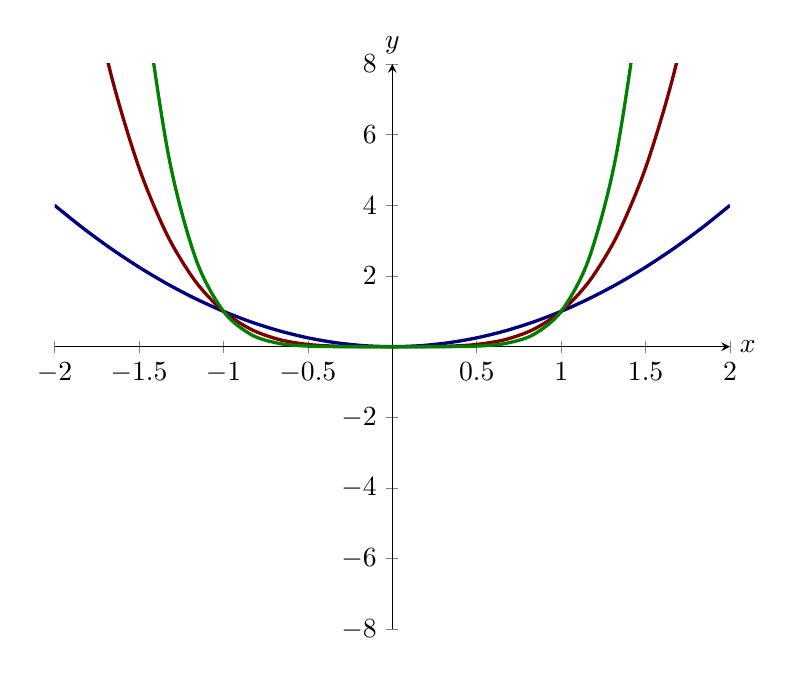
\begin{tikzpicture}
        			\begin{axis}[
          			domain=-2:2,
          			xmin=-2, xmax=2,
          			ymin=-8, ymax=8,
          			width=4in,
          			axis lines =middle, xlabel=$x$, ylabel=$y$,
          			every axis y label/.style={at=(current axis.above origin),anchor=south},
          			every axis x label/.style={at=(current axis.right of origin),anchor=west},
          			]
	 	 		\addplot [very thick, penColor, smooth] {x^2};
				\addplot [very thick, penColor2, smooth] {x^4};
				\addplot [very thick, penColor4, smooth] {x^6};
        			\end{axis}
      		\end{tikzpicture}
	\end{center}

	
Here are the graphs of $f(x)=x^n$ for $n = 3$, $5$, and $7$:
	\begin{center}
		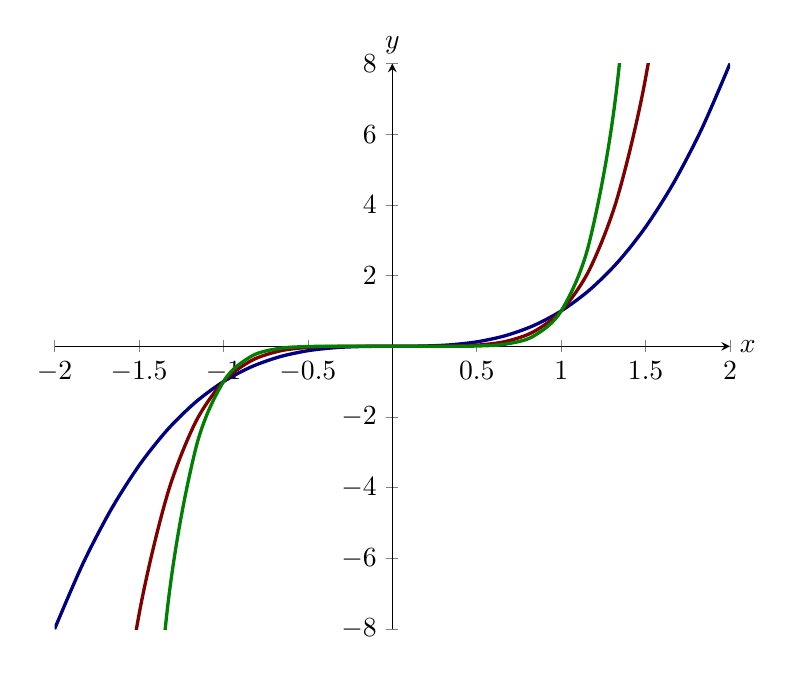
\begin{tikzpicture}
        			\begin{axis}[
          			domain=-2:2,
          			xmin=-2, xmax=2,
          			ymin=-8, ymax=8,
          			width=4in,
          			axis lines =middle, xlabel=$x$, ylabel=$y$,
          			every axis y label/.style={at=(current axis.above origin),anchor=south},
          			every axis x label/.style={at=(current axis.right of origin),anchor=west},
          			]
	 	 		\addplot [very thick, penColor, smooth] {x^3};
				\addplot [very thick, penColor2, smooth] {x^5};
				\addplot [very thick, penColor4, smooth] {x^7};
        			\end{axis}
      		\end{tikzpicture}
	\end{center}

Notice the similarity between the all the graphs with $n$ even.  They all have the same basic cup shape, but higher values of $n$ make the graphs flatter in $(-1,1)$ and steeper outside $(-1,1)$.

The same thing happens with the $n$ odd graphs.  They have the same basic shape, but higher values of $n$ make the graphs flatter near the origin and steeper past $1$ and $-1$.

When $n$ is even, what is happening to the output values of $f(x) = x^n$ as $x$ gets larger and larger?  They themselves get larger and larger!  As $x$ increases without bound, so do the outputs.
The same thing happens as $x$ gets larger and larger in the negative direction without bound.  This is the end behavior we were looking for.  We'll say it this way:

\begin{align*}
	\text{As} \quad x \to \infty \, ,  \quad & x^n \to \infty \\
	\text{As} \quad x \to -\infty \, , \quad & x^n \to \infty \quad \text{, for $n$ even}
\end{align*}

For $n$ odd we have a slightly different end behavior.
\begin{align*}
	\text{As} \quad x \to \infty \, ,  \quad & x^n \to \infty \\
	\text{As} \quad x \to -\infty \, , \quad & x^n \to -\infty \quad \text{, for $n$ odd}
\end{align*}

Next we need to see how a coefficient could change this.  Remember how multiplying by a constant transforms a graph?  If the constant is positive the graph is vertically stretched/compressed.
If the constant is negative the graph is flipped over the $x$-axis and then vertically stretched/compressed.  This means if the coefficient of $x^n$ is positive, the end behavior is unaffected.  If the 
coefficient is negative, the end behavior is negated as well.

\begin{example}
	Find the end behavior of $f(x) = -3x^4$.
	\begin{explanation}
		Since $4$ is even, the function $x^4$ has end behavior 
		\begin{align*}
			\text{As} \quad x \to \infty \, ,  \quad & x^4 \to \infty \\
			\text{As} \quad x \to -\infty \, , \quad & x^4 \to \infty 
		\end{align*}
		The coefficient is negative, changing our end behavior to
		\begin{align*}
			\text{As} \quad x \to \infty \, ,  \quad & -3x^4 \to -\infty \\
			\text{As} \quad x \to -\infty \, , \quad & -3x^4 \to -\infty 
		\end{align*}
	\end{explanation}
\end{example}

\begin{problem}
	Find the end behavior of $g(x) = -6 x^9$.
	\begin{align*}
		\text{As} \quad x \to \infty \, ,  \quad & -6x^9 \to \answer{-\infty} \\
		\text{As} \quad x \to -\infty \, , \quad & -6x^9 \to \answer{\infty} 
	\end{align*}
\end{problem}


We understand monomials.  What about more general polynomials? 
\begin{example}
	Find the end behavior of $f(x) = 3x^5 - 4x^3 + 1$.
	\begin{explanation}
		If we rewrite the function as:
		\begin{align*}
			f(x) &= 3x^5 - 4x^3 + 1 \\
				&= x^5 \left( \frac{3x^5}{x^5} - \frac{4x^3}{x^5} + \frac{1}{x^5} \right)\\
				&=x^5 \left( \frac{3x^5}{x^5} - \frac{4x^3}{x^5} + \frac{1}{x^5} \right)\\
				&= x^5 \left( 3 - \frac{4}{x^2} + \frac{1}{x^5} \right)
		\end{align*}
		Remember that as $x\to \pm\infty$ we saw that $x^2 \to \infty$ and that $x^5 \to \mp \infty$.  That means $\frac{4}{x^2} \to 0$ and $\frac{1}{x^5} \to 0$. 
		(We'll talk about this more when we talk about Rational Functions.)  This means everything in parentheses will basically be just $3$ as $x \to \pm \infty$.
		That is, the polynomial $3x^5 - 4x^3 + 1$ has the same end behavior as $3x^5$.  Thus
		\begin{align*}
			\text{As} \quad x \to \infty \, ,  \quad & f(x) \to \infty \\
			\text{As} \quad x \to -\infty \, , \quad & f(x) \to -\infty 
		\end{align*}
	\end{explanation}
\end{example}

This example showed us that \emph{the end behavior of a polynomial is the same as the end behavior of its leading term}.
\begin{problem}
	Find the end behavior of $g(x) = -6x^9 + 15x^5 + 7 x^4 - 18 x^3 + 91x^2 - 72 x + 4$
	\begin{align*}
		\text{As} \quad x \to \infty \, ,  \quad & g(x) \to \answer{-\infty} \\
		\text{As} \quad x \to -\infty \, , \quad & g(x) \to \answer{\infty} 
	\end{align*}
\end{problem}




\end{document}
